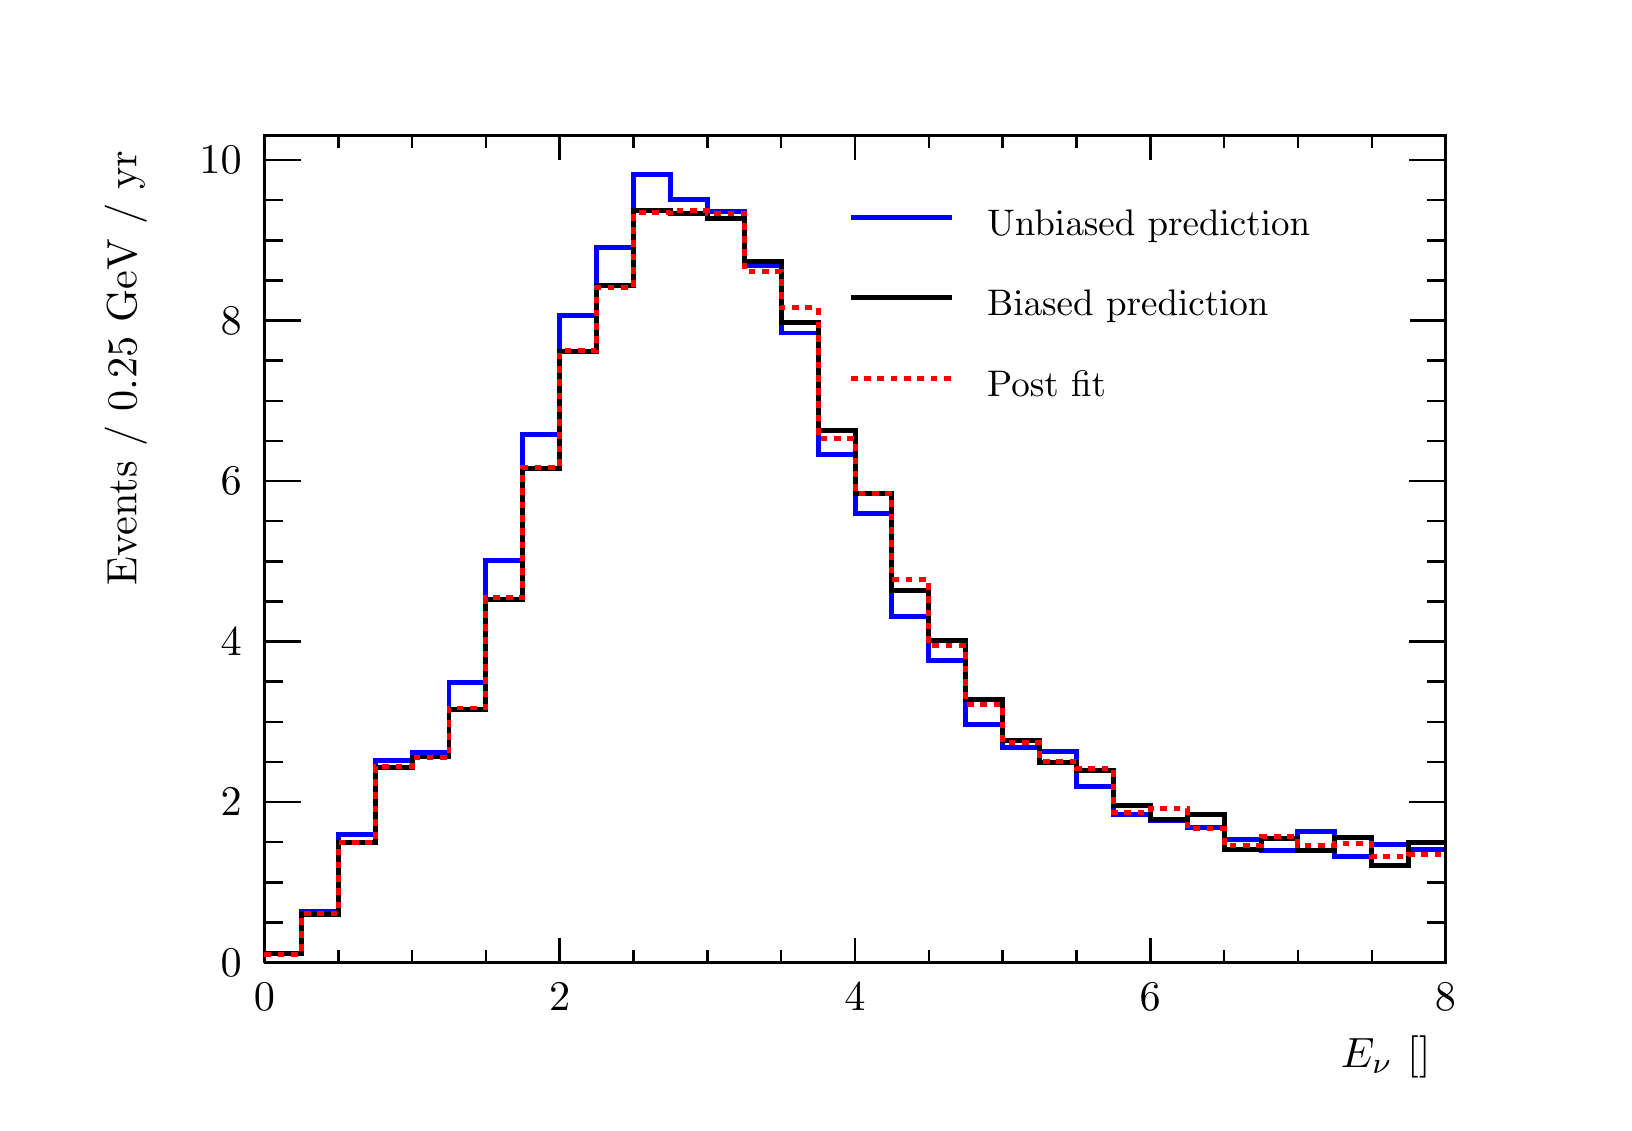
\begin{tikzpicture}
\pgfdeclareplotmark{cross} {
\pgfpathmoveto{\pgfpoint{-0.3\pgfplotmarksize}{\pgfplotmarksize}}
\pgfpathlineto{\pgfpoint{+0.3\pgfplotmarksize}{\pgfplotmarksize}}
\pgfpathlineto{\pgfpoint{+0.3\pgfplotmarksize}{0.3\pgfplotmarksize}}
\pgfpathlineto{\pgfpoint{+1\pgfplotmarksize}{0.3\pgfplotmarksize}}
\pgfpathlineto{\pgfpoint{+1\pgfplotmarksize}{-0.3\pgfplotmarksize}}
\pgfpathlineto{\pgfpoint{+0.3\pgfplotmarksize}{-0.3\pgfplotmarksize}}
\pgfpathlineto{\pgfpoint{+0.3\pgfplotmarksize}{-1.\pgfplotmarksize}}
\pgfpathlineto{\pgfpoint{-0.3\pgfplotmarksize}{-1.\pgfplotmarksize}}
\pgfpathlineto{\pgfpoint{-0.3\pgfplotmarksize}{-0.3\pgfplotmarksize}}
\pgfpathlineto{\pgfpoint{-1.\pgfplotmarksize}{-0.3\pgfplotmarksize}}
\pgfpathlineto{\pgfpoint{-1.\pgfplotmarksize}{0.3\pgfplotmarksize}}
\pgfpathlineto{\pgfpoint{-0.3\pgfplotmarksize}{0.3\pgfplotmarksize}}
\pgfpathclose
\pgfusepathqstroke
}
\pgfdeclareplotmark{cross*} {
\pgfpathmoveto{\pgfpoint{-0.3\pgfplotmarksize}{\pgfplotmarksize}}
\pgfpathlineto{\pgfpoint{+0.3\pgfplotmarksize}{\pgfplotmarksize}}
\pgfpathlineto{\pgfpoint{+0.3\pgfplotmarksize}{0.3\pgfplotmarksize}}
\pgfpathlineto{\pgfpoint{+1\pgfplotmarksize}{0.3\pgfplotmarksize}}
\pgfpathlineto{\pgfpoint{+1\pgfplotmarksize}{-0.3\pgfplotmarksize}}
\pgfpathlineto{\pgfpoint{+0.3\pgfplotmarksize}{-0.3\pgfplotmarksize}}
\pgfpathlineto{\pgfpoint{+0.3\pgfplotmarksize}{-1.\pgfplotmarksize}}
\pgfpathlineto{\pgfpoint{-0.3\pgfplotmarksize}{-1.\pgfplotmarksize}}
\pgfpathlineto{\pgfpoint{-0.3\pgfplotmarksize}{-0.3\pgfplotmarksize}}
\pgfpathlineto{\pgfpoint{-1.\pgfplotmarksize}{-0.3\pgfplotmarksize}}
\pgfpathlineto{\pgfpoint{-1.\pgfplotmarksize}{0.3\pgfplotmarksize}}
\pgfpathlineto{\pgfpoint{-0.3\pgfplotmarksize}{0.3\pgfplotmarksize}}
\pgfpathclose
\pgfusepathqfillstroke
}
\pgfdeclareplotmark{newstar} {
\pgfpathmoveto{\pgfqpoint{0pt}{\pgfplotmarksize}}
\pgfpathlineto{\pgfqpointpolar{44}{0.5\pgfplotmarksize}}
\pgfpathlineto{\pgfqpointpolar{18}{\pgfplotmarksize}}
\pgfpathlineto{\pgfqpointpolar{-20}{0.5\pgfplotmarksize}}
\pgfpathlineto{\pgfqpointpolar{-54}{\pgfplotmarksize}}
\pgfpathlineto{\pgfqpointpolar{-90}{0.5\pgfplotmarksize}}
\pgfpathlineto{\pgfqpointpolar{234}{\pgfplotmarksize}}
\pgfpathlineto{\pgfqpointpolar{198}{0.5\pgfplotmarksize}}
\pgfpathlineto{\pgfqpointpolar{162}{\pgfplotmarksize}}
\pgfpathlineto{\pgfqpointpolar{134}{0.5\pgfplotmarksize}}
\pgfpathclose
\pgfusepathqstroke
}
\pgfdeclareplotmark{newstar*} {
\pgfpathmoveto{\pgfqpoint{0pt}{\pgfplotmarksize}}
\pgfpathlineto{\pgfqpointpolar{44}{0.5\pgfplotmarksize}}
\pgfpathlineto{\pgfqpointpolar{18}{\pgfplotmarksize}}
\pgfpathlineto{\pgfqpointpolar{-20}{0.5\pgfplotmarksize}}
\pgfpathlineto{\pgfqpointpolar{-54}{\pgfplotmarksize}}
\pgfpathlineto{\pgfqpointpolar{-90}{0.5\pgfplotmarksize}}
\pgfpathlineto{\pgfqpointpolar{234}{\pgfplotmarksize}}
\pgfpathlineto{\pgfqpointpolar{198}{0.5\pgfplotmarksize}}
\pgfpathlineto{\pgfqpointpolar{162}{\pgfplotmarksize}}
\pgfpathlineto{\pgfqpointpolar{134}{0.5\pgfplotmarksize}}
\pgfpathclose
\pgfusepathqfillstroke
}
\definecolor{c}{rgb}{1,1,1};
\draw [color=c, fill=c] (0,0) rectangle (20,13.639);
\draw [color=c, fill=c] (3,1.77307) rectangle (18,12.2751);
\definecolor{c}{rgb}{0,0,0};
\draw [c,line width=0.9] (3,1.77307) -- (3,12.2751) -- (18,12.2751) -- (18,1.77307) -- (3,1.77307);
\definecolor{c}{rgb}{1,1,1};
\draw [color=c, fill=c] (3,1.77307) rectangle (18,12.2751);
\definecolor{c}{rgb}{0,0,0};
\draw [c,line width=0.9] (3,1.77307) -- (3,12.2751) -- (18,12.2751) -- (18,1.77307) -- (3,1.77307);
\definecolor{c}{rgb}{0,0,1};
\draw [c,line width=1.8] (3,1.88189) -- (3.46875,1.88189) -- (3.46875,2.42765) -- (3.9375,2.42765) -- (3.9375,3.39902) -- (4.40625,3.39902) -- (4.40625,4.34076) -- (4.875,4.34076) -- (4.875,4.43946) -- (5.34375,4.43946) -- (5.34375,5.32589) --
 (5.8125,5.32589) -- (5.8125,6.88053) -- (6.28125,6.88053) -- (6.28125,8.48165) -- (6.75,8.48165) -- (6.75,9.99191) -- (7.21875,9.99191) -- (7.21875,10.857) -- (7.6875,10.857) -- (7.6875,11.775) -- (8.15625,11.775) -- (8.15625,11.468) --
 (8.625,11.468) -- (8.625,11.3108) -- (9.09375,11.3108) -- (9.09375,10.6287) -- (9.5625,10.6287) -- (9.5625,9.76823) -- (10.0312,9.76823) -- (10.0312,8.2256) -- (10.5,8.2256) -- (10.5,7.47415) -- (10.9688,7.47415) -- (10.9688,6.16562) --
 (11.4375,6.16562) -- (11.4375,5.60397) -- (11.9062,5.60397) -- (11.9062,4.79174) -- (12.375,4.79174) -- (12.375,4.50955) -- (12.8438,4.50955) -- (12.8438,4.4548) -- (13.3125,4.4548) -- (13.3125,4.01262) -- (13.7812,4.01262) -- (13.7812,3.6593) --
 (14.25,3.6593) -- (14.25,3.57943) -- (14.7188,3.57943) -- (14.7188,3.48817) -- (15.1875,3.48817) -- (15.1875,3.33923) -- (15.6562,3.33923) -- (15.6562,3.20042) -- (16.125,3.20042) -- (16.125,3.44332) -- (16.5938,3.44332) -- (16.5938,3.11861) --
 (17.0625,3.11861) -- (17.0625,3.27712) -- (17.5312,3.27712) -- (17.5312,3.21237) -- (18,3.21237);
\definecolor{c}{rgb}{0,0,0};
\draw [c,line width=0.9] (3,1.77307) -- (18,1.77307);
\draw [c,line width=0.9] (3,2.07994) -- (3,1.77307);
\draw [c,line width=0.9] (3.9375,1.9265) -- (3.9375,1.77307);
\draw [c,line width=0.9] (4.875,1.9265) -- (4.875,1.77307);
\draw [c,line width=0.9] (5.8125,1.9265) -- (5.8125,1.77307);
\draw [c,line width=0.9] (6.75,2.07994) -- (6.75,1.77307);
\draw [c,line width=0.9] (7.6875,1.9265) -- (7.6875,1.77307);
\draw [c,line width=0.9] (8.625,1.9265) -- (8.625,1.77307);
\draw [c,line width=0.9] (9.5625,1.9265) -- (9.5625,1.77307);
\draw [c,line width=0.9] (10.5,2.07994) -- (10.5,1.77307);
\draw [c,line width=0.9] (11.4375,1.9265) -- (11.4375,1.77307);
\draw [c,line width=0.9] (12.375,1.9265) -- (12.375,1.77307);
\draw [c,line width=0.9] (13.3125,1.9265) -- (13.3125,1.77307);
\draw [c,line width=0.9] (14.25,2.07994) -- (14.25,1.77307);
\draw [c,line width=0.9] (15.1875,1.9265) -- (15.1875,1.77307);
\draw [c,line width=0.9] (16.125,1.9265) -- (16.125,1.77307);
\draw [c,line width=0.9] (17.0625,1.9265) -- (17.0625,1.77307);
\draw [c,line width=0.9] (18,2.07994) -- (18,1.77307);
\draw [anchor=base] (3,1.15931) node[scale=1.52731, color=c, rotate=0]{0};
\draw [anchor=base] (6.75,1.15931) node[scale=1.52731, color=c, rotate=0]{2};
\draw [anchor=base] (10.5,1.15931) node[scale=1.52731, color=c, rotate=0]{4};
\draw [anchor=base] (14.25,1.15931) node[scale=1.52731, color=c, rotate=0]{6};
\draw [anchor=base] (18,1.15931) node[scale=1.52731, color=c, rotate=0]{8};
\draw [anchor= east] (18,0.572837) node[scale=1.52731, color=c, rotate=0]{$E_{\nu}$ [\si{\GeV}]};
\draw [c,line width=0.9] (3,12.2751) -- (18,12.2751);
\draw [c,line width=0.9] (3,11.9682) -- (3,12.2751);
\draw [c,line width=0.9] (3.9375,12.1216) -- (3.9375,12.2751);
\draw [c,line width=0.9] (4.875,12.1216) -- (4.875,12.2751);
\draw [c,line width=0.9] (5.8125,12.1216) -- (5.8125,12.2751);
\draw [c,line width=0.9] (6.75,11.9682) -- (6.75,12.2751);
\draw [c,line width=0.9] (7.6875,12.1216) -- (7.6875,12.2751);
\draw [c,line width=0.9] (8.625,12.1216) -- (8.625,12.2751);
\draw [c,line width=0.9] (9.5625,12.1216) -- (9.5625,12.2751);
\draw [c,line width=0.9] (10.5,11.9682) -- (10.5,12.2751);
\draw [c,line width=0.9] (11.4375,12.1216) -- (11.4375,12.2751);
\draw [c,line width=0.9] (12.375,12.1216) -- (12.375,12.2751);
\draw [c,line width=0.9] (13.3125,12.1216) -- (13.3125,12.2751);
\draw [c,line width=0.9] (14.25,11.9682) -- (14.25,12.2751);
\draw [c,line width=0.9] (15.1875,12.1216) -- (15.1875,12.2751);
\draw [c,line width=0.9] (16.125,12.1216) -- (16.125,12.2751);
\draw [c,line width=0.9] (17.0625,12.1216) -- (17.0625,12.2751);
\draw [c,line width=0.9] (18,11.9682) -- (18,12.2751);
\draw [c,line width=0.9] (3,1.77307) -- (3,12.2751);
\draw [c,line width=0.9] (3.462,1.77307) -- (3,1.77307);
\draw [c,line width=0.9] (3.231,2.2826) -- (3,2.2826);
\draw [c,line width=0.9] (3.231,2.79213) -- (3,2.79213);
\draw [c,line width=0.9] (3.231,3.30167) -- (3,3.30167);
\draw [c,line width=0.9] (3.462,3.8112) -- (3,3.8112);
\draw [c,line width=0.9] (3.231,4.32074) -- (3,4.32074);
\draw [c,line width=0.9] (3.231,4.83027) -- (3,4.83027);
\draw [c,line width=0.9] (3.231,5.33981) -- (3,5.33981);
\draw [c,line width=0.9] (3.462,5.84934) -- (3,5.84934);
\draw [c,line width=0.9] (3.231,6.35887) -- (3,6.35887);
\draw [c,line width=0.9] (3.231,6.86841) -- (3,6.86841);
\draw [c,line width=0.9] (3.231,7.37794) -- (3,7.37794);
\draw [c,line width=0.9] (3.462,7.88748) -- (3,7.88748);
\draw [c,line width=0.9] (3.231,8.39701) -- (3,8.39701);
\draw [c,line width=0.9] (3.231,8.90655) -- (3,8.90655);
\draw [c,line width=0.9] (3.231,9.41608) -- (3,9.41608);
\draw [c,line width=0.9] (3.462,9.92561) -- (3,9.92561);
\draw [c,line width=0.9] (3.231,10.4351) -- (3,10.4351);
\draw [c,line width=0.9] (3.231,10.9447) -- (3,10.9447);
\draw [c,line width=0.9] (3.231,11.4542) -- (3,11.4542);
\draw [c,line width=0.9] (3.462,11.9638) -- (3,11.9638);
\draw [c,line width=0.9] (3.462,11.9638) -- (3,11.9638);
\draw [anchor= east] (2.9,1.77307) node[scale=1.52731, color=c, rotate=0]{0};
\draw [anchor= east] (2.9,3.8112) node[scale=1.52731, color=c, rotate=0]{2};
\draw [anchor= east] (2.9,5.84934) node[scale=1.52731, color=c, rotate=0]{4};
\draw [anchor= east] (2.9,7.88748) node[scale=1.52731, color=c, rotate=0]{6};
\draw [anchor= east] (2.9,9.92561) node[scale=1.52731, color=c, rotate=0]{8};
\draw [anchor= east] (2.9,11.9638) node[scale=1.52731, color=c, rotate=0]{10};
\draw [anchor= east] (1.24,12.2751) node[scale=1.52731, color=c, rotate=90]{Events / 0.25 GeV / yr};
\draw [c,line width=0.9] (18,1.77307) -- (18,12.2751);
\draw [c,line width=0.9] (17.538,1.77307) -- (18,1.77307);
\draw [c,line width=0.9] (17.769,2.2826) -- (18,2.2826);
\draw [c,line width=0.9] (17.769,2.79213) -- (18,2.79213);
\draw [c,line width=0.9] (17.769,3.30167) -- (18,3.30167);
\draw [c,line width=0.9] (17.538,3.8112) -- (18,3.8112);
\draw [c,line width=0.9] (17.769,4.32074) -- (18,4.32074);
\draw [c,line width=0.9] (17.769,4.83027) -- (18,4.83027);
\draw [c,line width=0.9] (17.769,5.33981) -- (18,5.33981);
\draw [c,line width=0.9] (17.538,5.84934) -- (18,5.84934);
\draw [c,line width=0.9] (17.769,6.35887) -- (18,6.35887);
\draw [c,line width=0.9] (17.769,6.86841) -- (18,6.86841);
\draw [c,line width=0.9] (17.769,7.37794) -- (18,7.37794);
\draw [c,line width=0.9] (17.538,7.88748) -- (18,7.88748);
\draw [c,line width=0.9] (17.769,8.39701) -- (18,8.39701);
\draw [c,line width=0.9] (17.769,8.90655) -- (18,8.90655);
\draw [c,line width=0.9] (17.769,9.41608) -- (18,9.41608);
\draw [c,line width=0.9] (17.538,9.92561) -- (18,9.92561);
\draw [c,line width=0.9] (17.769,10.4351) -- (18,10.4351);
\draw [c,line width=0.9] (17.769,10.9447) -- (18,10.9447);
\draw [c,line width=0.9] (17.769,11.4542) -- (18,11.4542);
\draw [c,line width=0.9] (17.538,11.9638) -- (18,11.9638);
\draw [c,line width=0.9] (17.538,11.9638) -- (18,11.9638);
\draw [c,line width=1.8] (3,1.88189) -- (3.46875,1.88189) -- (3.46875,2.38057) -- (3.9375,2.38057) -- (3.9375,3.29559) -- (4.40625,3.29559) -- (4.40625,4.2494) -- (4.875,4.2494) -- (4.875,4.3836) -- (5.34375,4.3836) -- (5.34375,4.99052) --
 (5.8125,4.99052) -- (5.8125,6.38756) -- (6.28125,6.38756) -- (6.28125,8.04822) -- (6.75,8.04822) -- (6.75,9.53617) -- (7.21875,9.53617) -- (7.21875,10.3672) -- (7.6875,10.3672) -- (7.6875,11.3195) -- (8.15625,11.3195) -- (8.15625,11.2825) --
 (8.625,11.2825) -- (8.625,11.2256) -- (9.09375,11.2256) -- (9.09375,10.6794) -- (9.5625,10.6794) -- (9.5625,9.90518) -- (10.0312,9.90518) -- (10.0312,8.53361) -- (10.5,8.53361) -- (10.5,7.73312) -- (10.9688,7.73312) -- (10.9688,6.50233) --
 (11.4375,6.50233) -- (11.4375,5.86186) -- (11.9062,5.86186) -- (11.9062,5.1107) -- (12.375,5.1107) -- (12.375,4.59266) -- (12.8438,4.59266) -- (12.8438,4.314) -- (13.3125,4.314) -- (13.3125,4.20893) -- (13.7812,4.20893) -- (13.7812,3.77033) --
 (14.25,3.77033) -- (14.25,3.58809) -- (14.7188,3.58809) -- (14.7188,3.65788) -- (15.1875,3.65788) -- (15.1875,3.20305) -- (15.6562,3.20305) -- (15.6562,3.34356) -- (16.125,3.34356) -- (16.125,3.20205) -- (16.5938,3.20205) -- (16.5938,3.36564) --
 (17.0625,3.36564) -- (17.0625,3.00178) -- (17.5312,3.00178) -- (17.5312,3.29841) -- (18,3.29841);
\definecolor{c}{rgb}{1,0,0};
\draw [c,dash pattern=on 2.40pt off 2.40pt ,line width=1.8] (3,1.88148) -- (3.46875,1.88148) -- (3.46875,2.39093) -- (3.9375,2.39093) -- (3.9375,3.29919) -- (4.40625,3.29919) -- (4.40625,4.26338) -- (4.875,4.26338) -- (4.875,4.37426) --
 (5.34375,4.37426) -- (5.34375,5.00582) -- (5.8125,5.00582) -- (5.8125,6.40347) -- (6.28125,6.40347) -- (6.28125,8.06436) -- (6.75,8.06436) -- (6.75,9.54058) -- (7.21875,9.54058) -- (7.21875,10.3421) -- (7.6875,10.3421) -- (7.6875,11.2934) --
 (8.15625,11.2934) -- (8.15625,11.3219) -- (8.625,11.3219) -- (8.625,11.2914) -- (9.09375,11.2914) -- (9.09375,10.5494) -- (9.5625,10.5494) -- (9.5625,10.0865) -- (10.0312,10.0865) -- (10.0312,8.42467) -- (10.5,8.42467) -- (10.5,7.72755) --
 (10.9688,7.72755) -- (10.9688,6.63834) -- (11.4375,6.63834) -- (11.4375,5.79508) -- (11.9062,5.79508) -- (11.9062,5.05644) -- (12.375,5.05644) -- (12.375,4.57255) -- (12.8438,4.57255) -- (12.8438,4.33257) -- (13.3125,4.33257) -- (13.3125,4.23454) --
 (13.7812,4.23454) -- (13.7812,3.67941) -- (14.25,3.67941) -- (14.25,3.72731) -- (14.7188,3.72731) -- (14.7188,3.47009) -- (15.1875,3.47009) -- (15.1875,3.25757) -- (15.6562,3.25757) -- (15.6562,3.37092) -- (16.125,3.37092) -- (16.125,3.25706) --
 (16.5938,3.25706) -- (16.5938,3.28182) -- (17.0625,3.28182) -- (17.0625,3.12204) -- (17.5312,3.12204) -- (17.5312,3.14337) -- (18,3.14337);
\definecolor{c}{rgb}{1,1,1};
\draw [color=c, fill=c] (10.1719,8.68195) rectangle (17.5358,11.7479);
\definecolor{c}{rgb}{0,0,0};
\draw [anchor=base west] (12.0129,11.0069) node[scale=1.3364, color=c, rotate=0]{Unbiased prediction};
\definecolor{c}{rgb}{0,0,1};
\draw [c,line width=1.8] (10.4481,11.2369) -- (11.7367,11.2369);
\definecolor{c}{rgb}{0,0,0};
\draw [anchor=base west] (12.0129,9.98496) node[scale=1.3364, color=c, rotate=0]{Biased prediction};
\draw [c,line width=1.8] (10.4481,10.2149) -- (11.7367,10.2149);
\draw [anchor=base west] (12.0129,8.96299) node[scale=1.3364, color=c, rotate=0]{Post fit};
\definecolor{c}{rgb}{1,0,0};
\draw [c,dash pattern=on 2.40pt off 2.40pt ,line width=1.8] (10.4481,9.19293) -- (11.7367,9.19293);
\end{tikzpicture}
